\PassOptionsToPackage{top=3cm,left=3cm,right=3cm,bottom=3cm}{geometry}
\documentclass[fleqn,11pt]{wlscirep}

\usepackage{import}
\usepackage{../paper/main-lancet}

\renewcommand{\paragraph}[1]{\vspace{0.3cm}\noindent\underline{\emph{#1}}\hfill\noindent}

\begin{document}

\doublespacing

\title{\bfseries\LARGE\singlespacing{Brief report: SARS-CoV-2 more frequently detected in indoor air than other respiratory viruses}}

% author list
\author[1,2]{Nicolas Banholzer}
\author[2,3]{Philipp Jent}
\author[2,4]{Pascal Bittel}
\author[1]{Kathrin Zürcher}
\author[4]{Lavinia Furrer}
\author[1]{Simon Bertschinger}
\author[5]{Ernest Weingartner}
\author[2,4]{Alban Ramette}
\author[1,6,7]{Matthias Egger}
\author[2,8]{Tina Hascher}
\author[1*,2]{Lukas Fenner}

\affil[1]{Institute of Social and Preventive Medicine, University of Bern, Bern, Switzerland}
\affil[2]{Multidisciplinary Center for Infectious Diseases, University of Bern, Bern, Switzerland}
\affil[3]{Department of Infectious Diseases, Inselspital, Bern University Hospital, University of Bern, Bern, Switzerland}
\affil[4]{Institute for Infectious Diseases, University of Bern, Bern, Switzerland}
\affil[5]{Institute for Sensors and Electronics, University of Applied Sciences and Arts Northwestern Switzerland, Windisch, Switzerland}
\affil[6]{Population Health Sciences, University of Bristol, Bristol, UK}
\affil[7]{Centre for Infectious Disease Epidemiology and Research, University of Cape Town, Cape Town, South Africa}
\affil[8]{Institute of Educational Science, University of Bern, Bern, Switzerland}

\affil[*]{Corresponding author: lukas.fenner@unibe.ch}


\vspace{2em}

%TC:ignore

\begin{information}\normalfont
\textbf{Word count:} Abstract 252, Manuscript 3,244 \\
\textbf{Display items:} Figure 1 \\
\textbf{References:} 37 \\
\textbf{Supporting information:} STROBE checklist, Supplementary Data with texts, tables, and figures
% \par
\end{information}

\begin{abstract}\normalfont
\noindent We compared air, air filters, and saliva samples from two studies conducted in winter 2021/2022 (during the SARS-CoV-2 omicron wave) and winter 2022/2023 (after the COVID-19 pandemic) in a Swiss school setting. Whereas during the pandemic we detected almost exclusively SARS-CoV-2 in human saliva (19~samples of SARS-CoV-2, 2~samples of non-SARS-CoV-2), the most common respiratory viruses after the pandemic were adenovirus, influenza~B, and rhinoviruses (3~samples of SARS-CoV-2, 47~samples of non-SARS-CoV-2). Despite the same study setting and environmental conditions, airborne detection of SARS-CoV-2 was relatively more frequent than the detection of non-SARS-CoV-2 viruses (10~samples of SARS-CoV-2 in 2021/2022 vs 2~samples of non-SARS-CoV-2 in 2022/2023). Our comparison suggests that respiratory viruses other than SARS-CoV-2 may be less detectable in the air and that close contact is required for transmission. \medskip

\par
\end{abstract}

\flushbottom
\maketitle

\vspace{2em}

\vspace{0.5em}

\noindent\textbf{Keywords:} respiratory viruses, airborne transmission, molecular detection
% maximum of 3-5 keywords

\thispagestyle{empty}
\sloppy
\raggedbottom

\newpage
%TC:endignore

\setcounter{page}{1}

%\section*{Introduction} 


\section*{Methods}

Data was collected in two classes of two secondary schools in winter 2021/2022 and two classrooms of one secondary school in winter 2022/2023 (age of students 14-17~years) in the canton of Solothurn, Switzerland, both over a seven-week study period from end of January to beginning of March. In winter 2021/2022, a general mask mandate was in place for the first 3~study weeks, followed by 2~weeks without intervention, and another 2~weeks of air cleaners installed in two classrooms. In winter 2022/2023, air cleaners were installed for half of the study period following a cross-over design. An air quality device (AQ Guard, Palas GmbH, Karlsruhe, Germany) continuously measured indoor CO$_2$ levels, temperature, and humidity in all classrooms. 

School classes participated in repetitive weekly (winter 2021/2022) and bi-weekly (winter 2022/2023) testing for a panel of respiratory infections. Airborne respiratory viruses were collected in each classroom with a cyclonic bioaerosol sampling device (Coriolis Micro Air, Bertin Instruments Montigny-le-Bretonneux, France) and a BioSpot-VIVAS condensation particle growth collection device (Aerosol Devices Inc., Ft. Collins, CO, USA)\cite{Lednicky2016AST}. The removable parts were regularly autoclaved. Finally, swabs from the air cleaners' HEPA filters were collected at the end of the study (winter 2021/2022) and after each intervention phase (winter 2022/2023). The HEPA filters were removed and divided into 20~fields. One sterile Phosphate-Buffered Saline-moistened swab per field was then taken for a total of 20~swabs per filter. Saliva and airborne samples were transported to the Institute of Infectious Diseases and stored at $-$80°C until further processing\cite{Huber2021}. 

Prior to the real-time (RT)-PCR analysis, daily bioaerosol samples were combined for each sampling device and filtered using Amicon Ultra-15 Centrifugal Filters with Ultracel 10,000 Dalton molecular weight cutoffs filters (UFC9010; MilliporeSigma, Burlington, USA) to a volume of 1\,mL. Saliva samples were analyzed directly without prior filtration. The Allplex RV Master Assay (Seegene, Seoul, South Korea) detects a panel of 19 major respiratory viruses and viral subtypes, including SARS-CoV-2, influenza, respiratory syncytial, metapneumovirus, adenovirus, rhinovirus, and parainfluenza. 

Descriptive statistics were utilized to depict differences in the type, number, and proportion of respiratory viruses between winter 2021/2022 and winter 2022/2023.

\section*{Results}

\section*{Discussion}

Furthermore, the distribution of respiratory viruses in this study was very different from that in our previous study. 

% why could we not detect so many bioaerosols

We detected fewer respiratory viruses in bioaerosol samples compared to our previous study\cite{Banholzer2023PLoSMed} (1~sample of adenovirus and 1~sample of rhinovirus in this study vs 10~samples of SARS-CoV-2 in the previous study), especially in relation to the number of positive saliva samples (50~samples in this study vs 21~in the previous study). Similarly, the number of viruses detected on the filters of the air cleaners was also lower in this study (4~positive samples in 160~swabs vs 8~positive samples in 80~swabs in the previous study). Importantly, there was a clear shift in the distribution of respiratory viruses in the current study compared to the previous study in 2022 during the SARS-CoV-2 Omicron variant. Whereas in 2022 we detected almost exclusively SARS-CoV-2 in human saliva, the most common respiratory viruses in 2023 were adenovirus, influenza~B, and rhinoviruses (only three SARS-CoV-2-positive samples). The shift in the pattern of respiratory viruses has been observed in other studies\cite{Nygaard2023Lancet,Sauteur2022EuroSurv}. 

% other reasons

Technical reasons for the differences in airborne detection are unlikely. The bioaerosol sampling devices and laboratory procedures were the same in both studies, and no technical problems were observed. Instead, airborne detection could have been influenced by environmental factors. Although temperature (overall between 19 and 25$^{\circ}$C) and relative humidity (overall between 25 and 50\%) were similar in both studies, the same levels may have different effects on the airborne survival of respiratory viruses. For example, airborne survival of rhinovirus and adenovirus increases with relative humidity, whereas the opposite relationship has been documented for influenza and SARS-CoV-2\cite{Tellier2009JTRSI,Ahlawat2020AAQR,Biryukov2020mS,Karim1985CJM,Davis1971AM}. A change in ventilation conditions could also have had a profound effect, but CO$_2$ levels were higher compared to the previous study (1,702$\pm$370\,ppm in this vs 1,064$\pm$232\,ppm in the previous study), suggesting that classrooms were not as well ventilated as during the COVID-19 pandemic. Although lower ventilation was partially offset by a greater reduction in aerosol and particle concentrations from air cleaners, the removal of particles by air cleaners may be slower than by natural ventilation.

% bioaerosol sampling in more depth

We speculate that the difference in airborne molecular detection of respiratory viruses between 2022 (pandemic) and 2023 (non-pandemic) is due to the different characteristics of the respiratory viruses. Differences in the physicochemical properties of virus-laden aerosols (\eg physical size, viral load, and infectivity), which influence the generation and survival of airborne viral RNA\cite{Wang2021,Sattar2016Book}, may facilitate the detection of SARS-CoV-2 in the air. The reason is that viral loads do often not exceed the detection limits of existing devices for bioaerosol sampling, which remains a challenge\cite{Wang2021,Belser2023PLOSPath,Bekking2019IORV,Mainelis2020AST}. For example, one study failed to detect any human rhinovirus in the exhaled breath of 16~HRV-infected subjects\cite{Fabian2011JAMPDD}. However, several studies showed that influenza\cite{Bischoff2013JID,Pan2017mSphere}, rhinovirus\cite{Myatt2004AJRCCM}, and adenovirus\cite{Nguyen2017OFID,Pan2017mSphere} can also be detected in airborne samples. Finally, the ability to detect pathogens in bioaerosols may be related to patient characteristics of the study participants. Several studies suggested an association between the generation of pathogenic aerosols and infectiousness\cite{Leung2020NatMed,Bischoff2013JID,Escombe2008PLoSMed}. Therefore, studies that include more infectious patients (intentionally or unintentionally) are likely to have a higher chance of detecting respiratory viruses in the air. 


\section{Comparison with previous study}\label{sec:comparison-prev-study}

% descriptive results

In a previous study\cite{Banholzer2023PLoSMed}, we estimated the effectiveness of mask wearing and air cleaners during the SARS-CoV-2 Omicron wave. \cref{fig:comparison} shows a comparison of the results. The distribution of respiratory infections is different (\cref{fig:comparison}a) because we almost exclusively detected SARS-CoV-2 in our previous study during the COVID-19 pandemic, as compared to a range of respiratory infections in this study during non-pandemic times. Although there were more positive saliva samples in this study, the number of respiratory infections detected in bioaerosols and on the HEPA-filters of the air cleaners was lower (\cref{fig:comparison}b).
The reductions in particle concentrations were larger and with lower uncertainty in this study (\cref{fig:comparison}c). The risk of infection tended to be lower with air cleaners in this study where air cleaners were analyzed using a cross-over design, but not in our previous study where air cleaners were installed only at the end of the study when most students had already been infected with SARS-Cov-2(\cref{fig:comparison}d).

% summary

To summarize, we found similar reductions in particle concentrations and a tendency for the relative risk of infection to be lower with air cleaners. To some extent, the differences between the two studies may be explained by different adjustments. While we could not adjust for ventilation in our previous study, the estimates in this study were adjusted for the daily air change rate, which correlated with the relative risk of infection (see \Cref{sec:detailed-molecular}). Furthermore, the distribution of respiratory viruses in this study was very different from that in our previous study and molecular airborne detection was lower.

\begin{figure}[!htpb]
    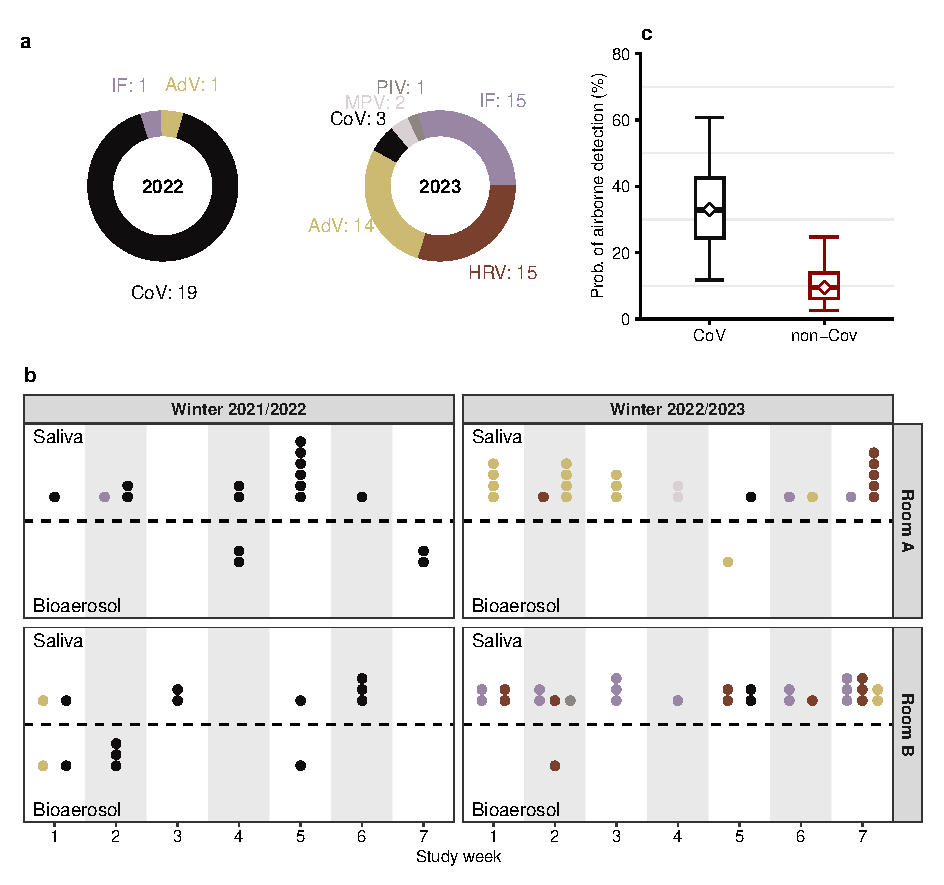
\includegraphics[width=\linewidth]{../../results/comparison.pdf} 
    \caption{\textbf{Comparison of the results between our previous study in 2022 during the COVID-19 pandemic (blue) and this study in 2023 during non-pandemic times (black).} \textbf{(a)}~Proportion of positive saliva samples by virus. Flu B: Influenza B, HRV: rhinovirus, AdV: adenovirus, CoV: SARS-CoV-2, MPV: metapneumovirus, PIV: parainfluenza virus. \textbf{(c)}~Estimated reduction in aerosol number and particle mass concentrations (CN in 1/cm$^3$) and particle mass concentration (PM for particles of sizes <1 to <10~$\mu$m, respectively in $\mu$gm$^{-3}$) with air cleaners (posterior mean as squares and 95\%-CrI as lines). \textbf{(d)}~Adjusted relative risk (ARR) of infection with air cleaners (posterior mean as squares and 95\%-CrI as lines).}
    \label{fig:comparison}
\end{figure}

% unlikely reasons for less airborne detection

Technical reasons for the differences in airborne detection are unlikely. The bioaerosol sampling devices and laboratory procedures were the same in both studies, and no technical problems were observed. Instead, airborne detection could have been influenced by environmental factors. Although temperature (overall between 19 and 25$^{\circ}$C) and relative humidity (overall between 25 and 50\%) were similar in both studies, the same levels may have different effects on the airborne survival of respiratory viruses. For example, airborne survival of rhinovirus and adenovirus increases with relative humidity, whereas the opposite relationship has been documented for influenza and SARS-CoV-2\cite{Tellier2009JTRSI,Ahlawat2020AAQR,Biryukov2020mS,Karim1985CJM,Davis1971AM}. A change in ventilation conditions could also have had a profound effect, but CO$_2$ levels were higher compared to the previous study (1,702$\pm$370\,ppm in this vs 1,064$\pm$232\,ppm in the previous study), suggesting that classrooms were not as well ventilated as during the COVID-19 pandemic. Although lower ventilation was partially offset by a greater reduction in aerosol and particle concentrations from air cleaners, the removal of particles by air cleaners may be slower than by natural ventilation. 

% likely reason for less airborne detection

More likely, SARS-CoV-2 may be easier to detect in the air due to physicochemical properties of virus-laden aerosols, so that its viral loads more often exceed the detection limits of existing devices for bioaerosol sampling,  which remains a challenge\cite{Wang2021,Belser2023PLOSPath,Bekking2019IORV,Mainelis2020AST}. For example, one study failed to detect any human rhinovirus in the exhaled breath of 16~HRV-infected subjects\cite{Fabian2011JAMPDD}. However, several studies showed that influenza\cite{Bischoff2013JID,Pan2017mSphere}, rhinovirus\cite{Myatt2004AJRCCM}, and adenovirus\cite{Nguyen2017OFID,Pan2017mSphere} can also be detected in airborne samples.

\bibliography{../paper/references.bib}

\end{document}